% Section 4: Results
% Note: \section{} header is in main.tex

\subsection{No Semantic Diversity Collapse}
\label{sec:no_collapse}

Reward-based curation does not cause semantic diversity collapse over three generations of iterative self-training. Table~\ref{tab:vendi_trajectory} reports Vendi Scores for all conditions across generations. Among the five curated configurations (C1--C4, C8), relative changes from Gen~0 to Gen~2 range from $-$0.27\% to $+$0.91\%, all within $\pm$1\%. This stability persists across every factor we vary: adaptation method (LoRA vs.\ Full-FT), candidate pool size ($K \in \{4, 8, 16\}$), and learning rate (5e-6 vs.\ 2e-5). C8, with the strongest selection pressure ($K{=}16$, 6.25\% retention), produces a change of only $-$0.19\%. Both Full-FT curated conditions (C3, C4) exhibit monotonically increasing Vendi Scores, while LoRA conditions remain flat or fluctuate transiently before recovery.

\begin{table}[t]
\centering
\small
\caption{Vendi Score across three self-training generations. $\Delta$ denotes relative change from Gen~0 to Gen~2. All curated conditions remain within $\pm$1\%, while random baselines show larger positive drift.}
\label{tab:vendi_trajectory}
\begin{tabular}{@{}llcccc@{}}
\toprule
& Config & Gen~0 & Gen~1 & Gen~2 & $\Delta$ (\%) \\
\midrule
\multicolumn{6}{@{}l}{\textit{Curated (ArmoRM top-1)}} \\
C1 & LoRA, $K{=}4$ & 107.54 & 106.73 & 107.25 & $-$0.27 \\
C2 & LoRA, $K{=}8$ & 107.21 & 107.26 & 107.25 & $+$0.04 \\
C3 & Full-FT, 5e-6 & 107.10 & 107.61 & 108.07 & $+$0.91 \\
C4 & Full-FT, 2e-5 & 107.81 & 108.03 & 108.54 & $+$0.68 \\
C8 & Full-FT, $K{=}16$ & 107.32 & 106.73 & 107.11 & $-$0.19 \\
\midrule
\multicolumn{6}{@{}l}{\textit{Random baseline (1-of-$K$)}} \\
C5 & LoRA, $K{=}4$ & 105.42 & 108.21 & 108.72 & $+$3.13 \\
C6 & Full-FT, 5e-6 & 107.17 & 107.87 & 108.64 & $+$1.37 \\
C7 & Full-FT, 2e-5 & 108.08 & 107.85 & 108.13 & $+$0.05 \\
\bottomrule
\end{tabular}
\end{table}

\begin{figure}[t]
\centering
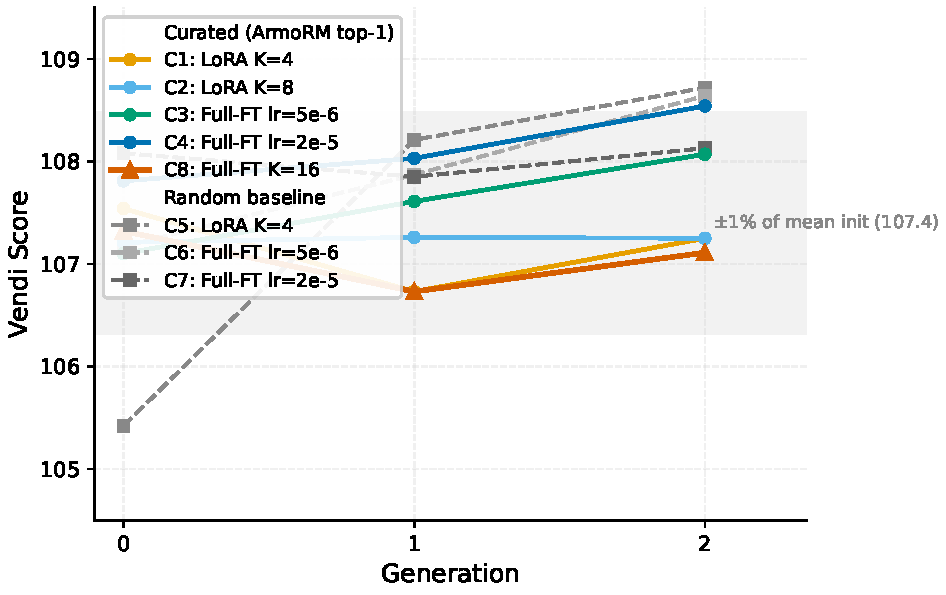
\includegraphics[width=\columnwidth]{figures/fig2_vendi_trajectories.pdf}
\caption{Vendi Score trajectories across three self-training generations for all 8 configurations. Curated conditions (solid lines) remain within $\pm$1\% of Gen~0, while random baselines (dashed) show larger positive drift.}
\label{fig:vendi_trajectories}
\end{figure}

Figure~\ref{fig:vendi_trajectories} visualizes these trajectories. Secondary metrics corroborate this result. Self-BLEU stays below 0.01 for all curated conditions (absolute values 0.002--0.009), and Self-BLEU-4 computed over full training corpora confirms this pattern (all conditions $<$0.016; Appendix~\ref{app:lexical_diversity}). Nearest-Neighbor Distance remains between 0.70 and 0.71 with no systematic contraction. These results contrast with predictions from the model collapse literature \cite{placeholder_shumailov, placeholder_alemohammad}. The critical difference is that each generation draws fresh stochastic samples ($T{=}0.7$) from the current model, and the prompt set provides a constant external anchor.

\subsection{Relative Suppression, Not Absolute Collapse}
\label{sec:suppression}

Curated conditions do not collapse, but they grow diversity more slowly than matched random baselines. C5 and C6 show Vendi Score increases of $+$3.13\% and $+$1.37\% (Table~\ref{tab:vendi_trajectory}), compared to $-$0.27\% and $+$0.91\% for their curated counterparts C1 and C3. This distinction matters: studies reporting that reward filtering reduces diversity relative to unfiltered baselines \cite{placeholder_kirk} are sometimes read as evidence of degeneration. Our data show that a curated model holding steady has not collapsed, even if an uncurated model drifted above it. Evaluating curation requires comparing each model against its own starting point, not against a diverging uncurated trajectory.

\subsection{Direction Reversal Across Training Regimes}
\label{sec:direction_reversal}

The curation gap (curated $\Delta$ minus random $\Delta$, in percentage points) reverses sign as training capacity increases. Under LoRA (C1 vs.\ C5), the gap is $-$3.40~pp. Under Full-FT at 5e-6 (C3 vs.\ C6), it contracts to $-$0.46~pp. Under Full-FT at 2e-5 (C4 vs.\ C7), it reverses to $+$0.63~pp: curation now promotes diversity (Figure~\ref{fig:direction_reversal}).

\begin{figure}[t]
\centering
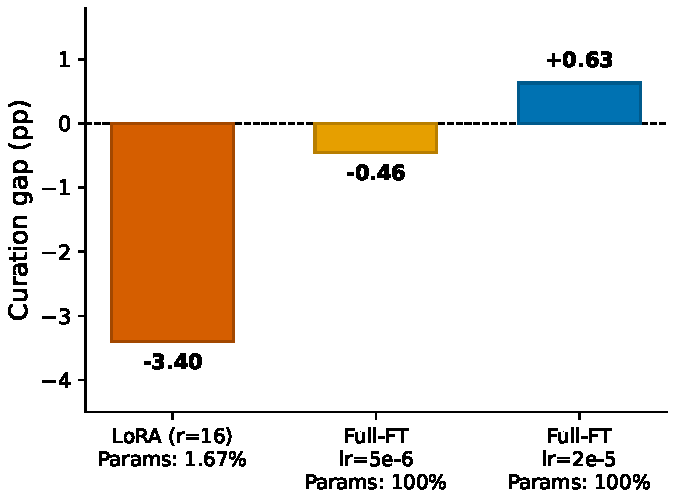
\includegraphics[width=\columnwidth]{figures/fig3_direction_reversal.pdf}
\caption{Curation gap (curated $\Delta$ minus random $\Delta$, in percentage points) across training regimes. The gap transitions from negative (curation suppresses diversity) under LoRA to positive (curation promotes diversity) under Full-FT with higher learning rate.}
\label{fig:direction_reversal}
\end{figure}

\begin{table}[t]
\centering
\small
\caption{Training loss per generation. LoRA conditions converge to similar final loss regardless of curation strategy. C8 ($K{=}16$) reaches the lowest Gen~2 loss (0.097).}
\label{tab:training_loss}
\begin{tabular}{@{}llccc@{}}
\toprule
& Config & Gen~0 & Gen~1 & Gen~2 \\
\midrule
C1 & LoRA, curated & 0.413 & 0.240 & 0.166 \\
C2 & LoRA ($K{=}8$), curated & 0.411 & 0.239 & 0.168 \\
C5 & LoRA, random & 0.407 & 0.224 & 0.152 \\
\midrule
C3 & Full-FT 5e-6, curated & 0.461 & 0.341 & 0.285 \\
C6 & Full-FT 5e-6, random & 0.461 & 0.335 & 0.277 \\
\midrule
C4 & Full-FT 2e-5, curated & 0.380 & 0.212 & 0.140 \\
C8 & Full-FT 2e-5, $K{=}16$ & 0.206 & 0.129 & \textbf{0.097} \\
C7 & Full-FT 2e-5, random & 0.377 & 0.199 & 0.132 \\
\bottomrule
\end{tabular}
\end{table}

Training loss trajectories (Table~\ref{tab:training_loss}) explain this reversal. Under LoRA, curated and random conditions converge to similar final loss (C1: 0.166, C5: 0.152). The rank-16 adapter's low-dimensional bottleneck limits how far any signal can reshape the output distribution. Random data, unconstrained by reward consistency, permits slightly more distributional drift within this bottleneck, producing the observed gap. Full-FT removes this constraint. At lr=2e-5, reward-selected data provides varied high-quality completions across topics that translate into greater semantic diversity when the model can fully absorb the curated distribution. The progression from LoRA through conservative Full-FT to aggressive Full-FT traces a continuum from parameter-limited to parameter-sufficient training.

This pattern is consistent with a capacity-mediated mechanism: LoRA's rank-16 bottleneck limits how much distributional structure the model can absorb, and the apparent suppression effect disappears when this constraint is removed. The practical implication is that experiments conducted exclusively with parameter-efficient methods may reach conclusions about curation's diversity impact that do not generalize to full fine-tuning.

\subsection{Quality-Diversity Non-Tradeoff}
\label{sec:quality_diversity}

Curation produces neither a quality gain large enough to motivate its use nor a diversity cost large enough to discourage it. Mean ArmoRM scores at Gen~2 range from 0.1096 (C5) to 0.1149 (C8), a spread of less than 5\%. All conditions show mild quality decreases from Gen~0 to Gen~2 ($-$0.3\% to $-$1.3\%; full per-generation scores in Table~\ref{tab:quality_scores}). The absence of meaningful quality improvement reflects saturation in the candidate quality distribution: the score gap between top-1 and average candidate is approximately 0.04, too narrow for the fine-tuned model to learn a meaningfully different quality level. The combined picture is that reward-based curation operates in a narrow effect regime at this scale: it does not collapse diversity, does not measurably improve quality, and its relative diversity effect depends more on training capacity than on curation strategy.
